%----------------------------------------------------------------------------------------
%   PHẦN 5: DEMO VÀ KẾT LUẬN
%----------------------------------------------------------------------------------------
\section{Demo và Kết luận}

%--- GIAO DIỆN HỆ THỐNG ---
\begin{frame}{Giao diện hệ thống}
    \begin{columns}
        \column{0.5\textwidth}
        \textbf{Tính năng chính:}
        \begin{itemize}
            \item Chọn video/camera đầu vào
            \item Cấu hình ROI (Stopline, Lanes)
            \item Chọn Pipeline ALPR
            \item Hiển thị real-time
            \item Xuất báo cáo vi phạm
        \end{itemize}

        \column{0.5\textwidth}
        \textbf{Thành phần UI:}
        \begin{itemize}
            \item Control Panel (bên trái)
            \item Video Display (giữa)
            \item Info Panel (bên phải)
            \item Status Bar (dưới)
        \end{itemize}
    \end{columns}

    \vspace{0.5em}
    \textit{Framework: PyQt5 + OpenCV}
\end{frame}

%--- KẾT QUẢ INFERENCE ---
\begin{frame}[allowframebreaks]{Kết quả Inference thực tế}
    \begin{figure}
        \centering
        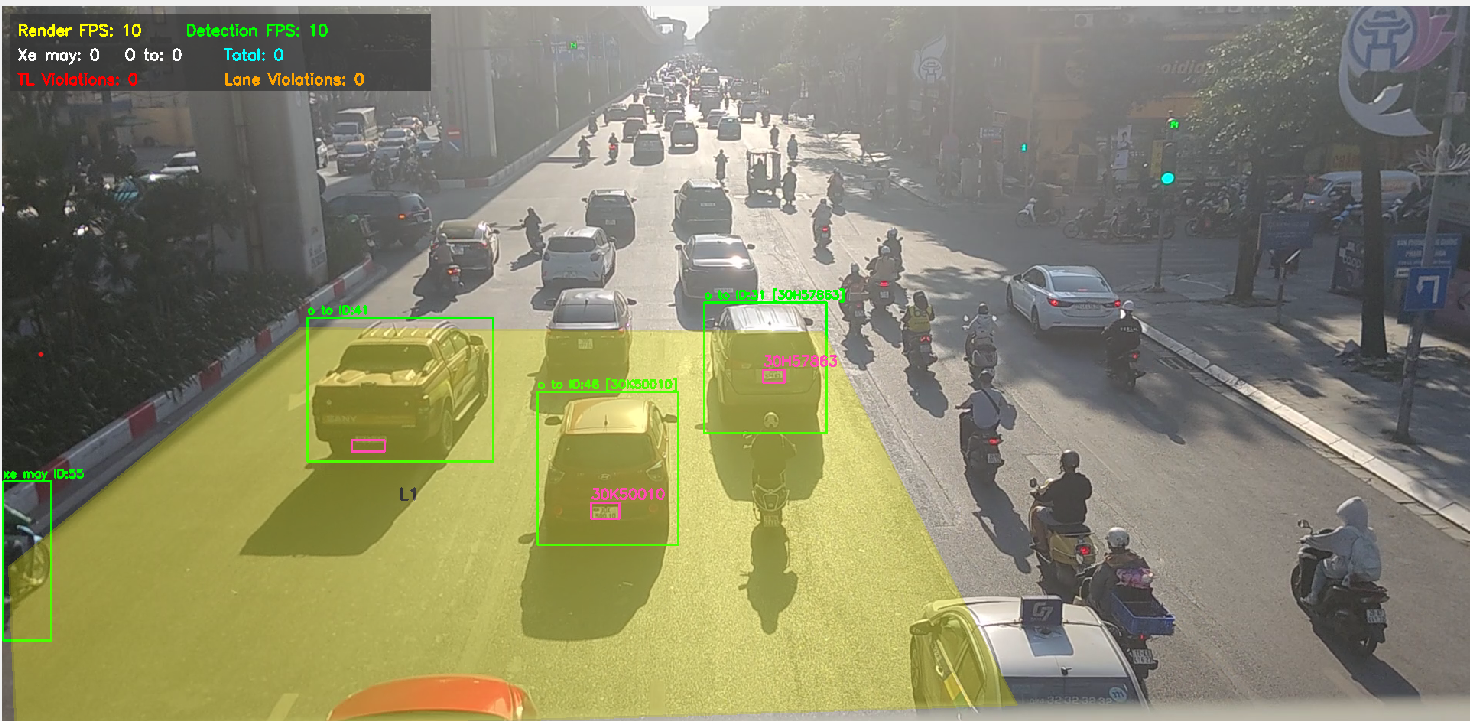
\includegraphics[width=0.85\linewidth]{Figures/plate_inference1.png}
        \caption{Pipeline 1: Phát hiện biển số chính xác}
    \end{figure}

    \framebreak

    \begin{figure}
        \centering
        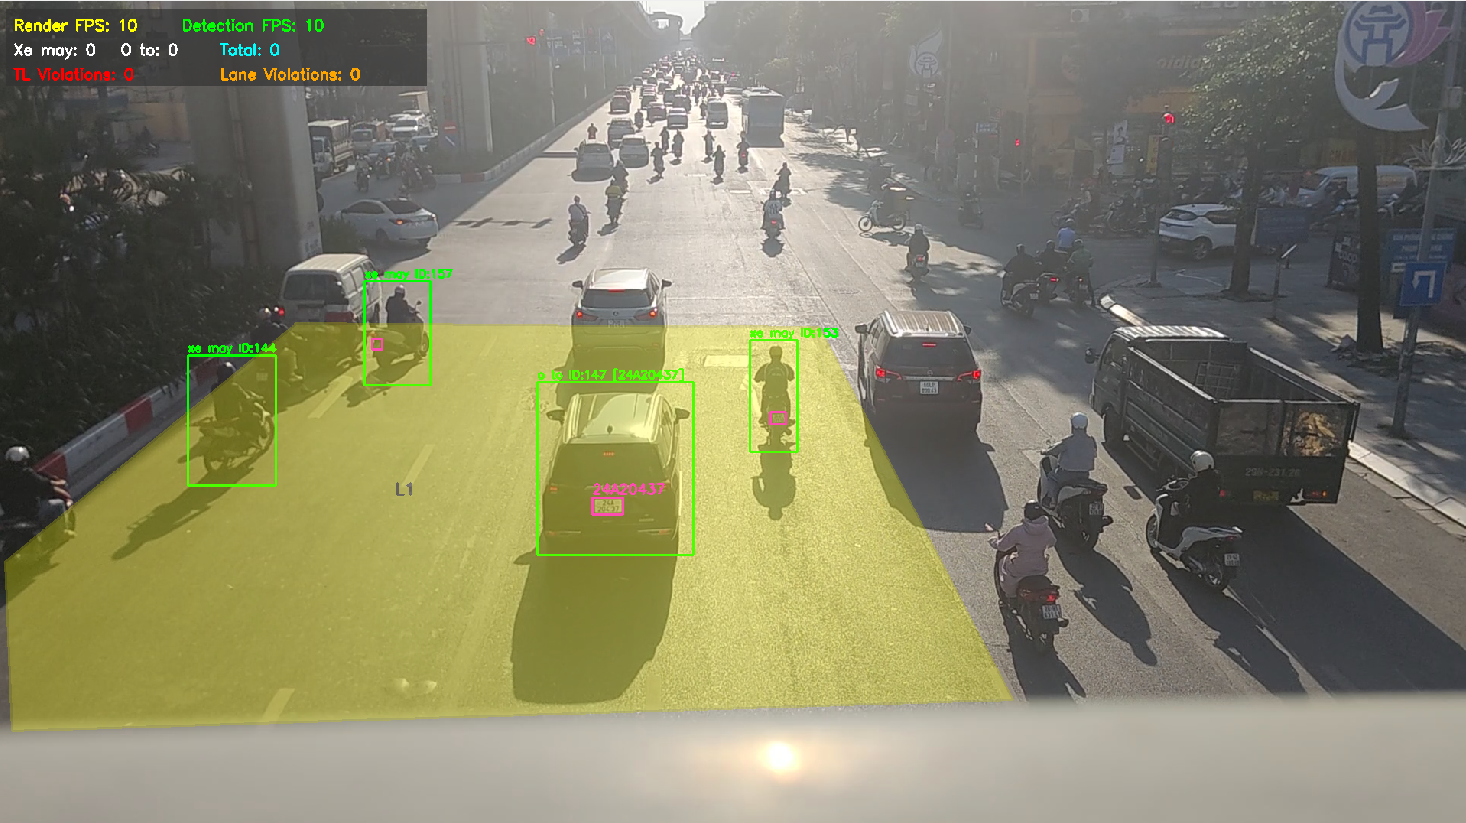
\includegraphics[width=0.85\linewidth]{Figures/plate_inference2.png}
        \caption{Pipeline 1: OCR nhận dạng biển số Việt Nam}
    \end{figure}

    \framebreak

    \begin{figure}
        \centering
        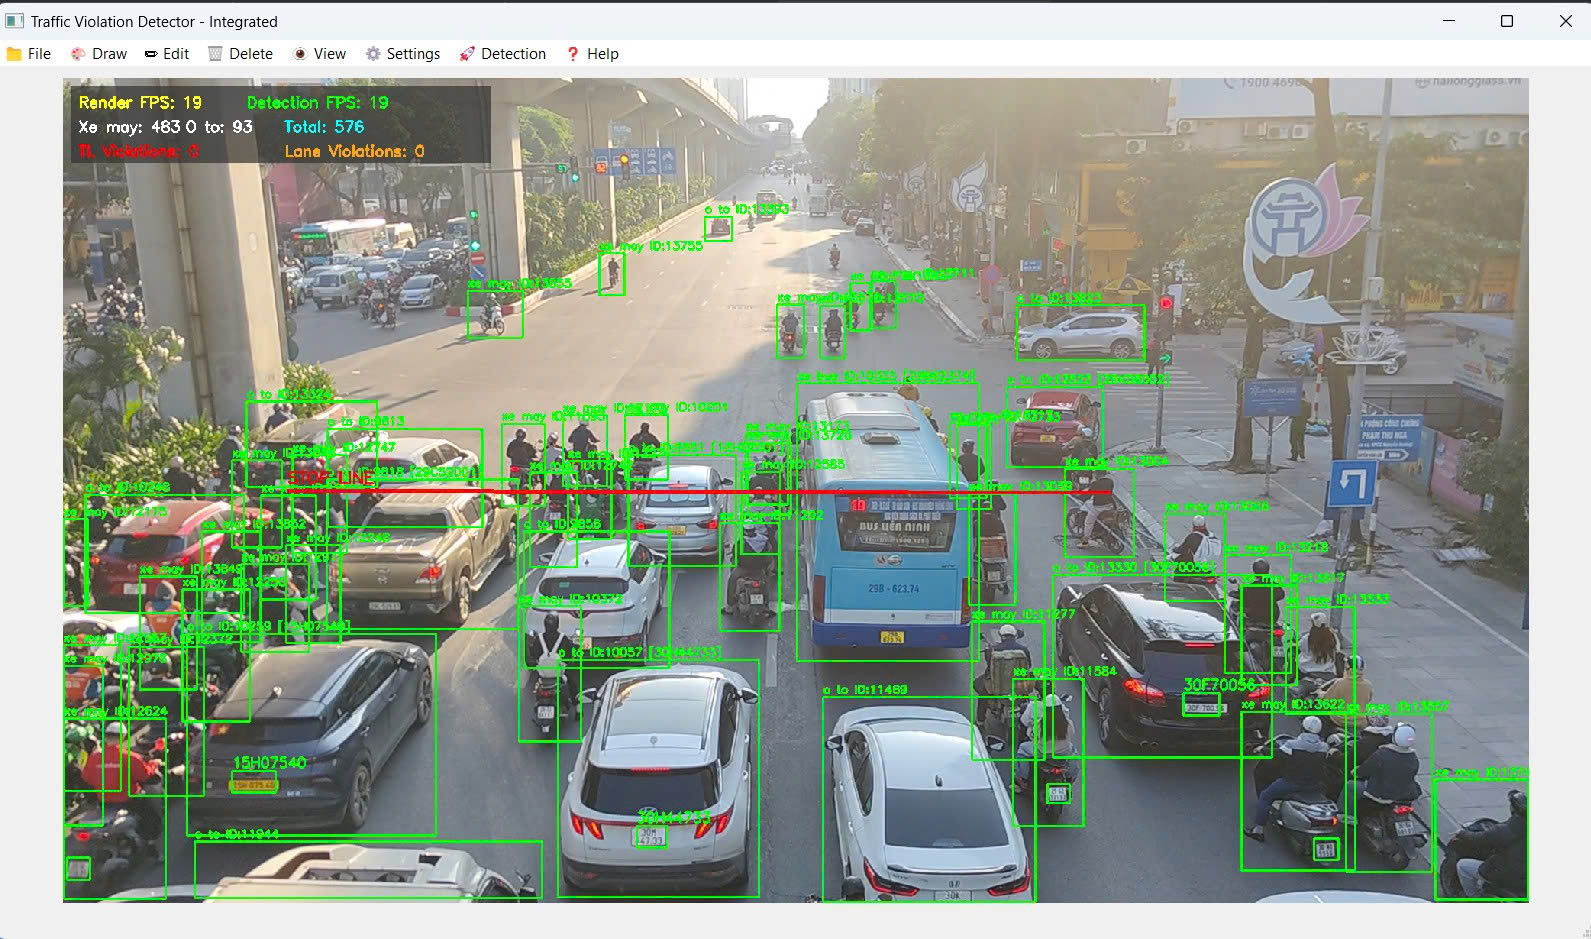
\includegraphics[width=0.85\linewidth]{Figures/ppthucnghiem2.jpg}
        \caption{Pipeline 2: Phát hiện đồng thời xe và biển số}
    \end{figure}
\end{frame}

%--- PHÁT HIỆN VI PHẠM ---
\begin{frame}[allowframebreaks]{Kết quả phát hiện vi phạm}
    \begin{figure}
        \centering
        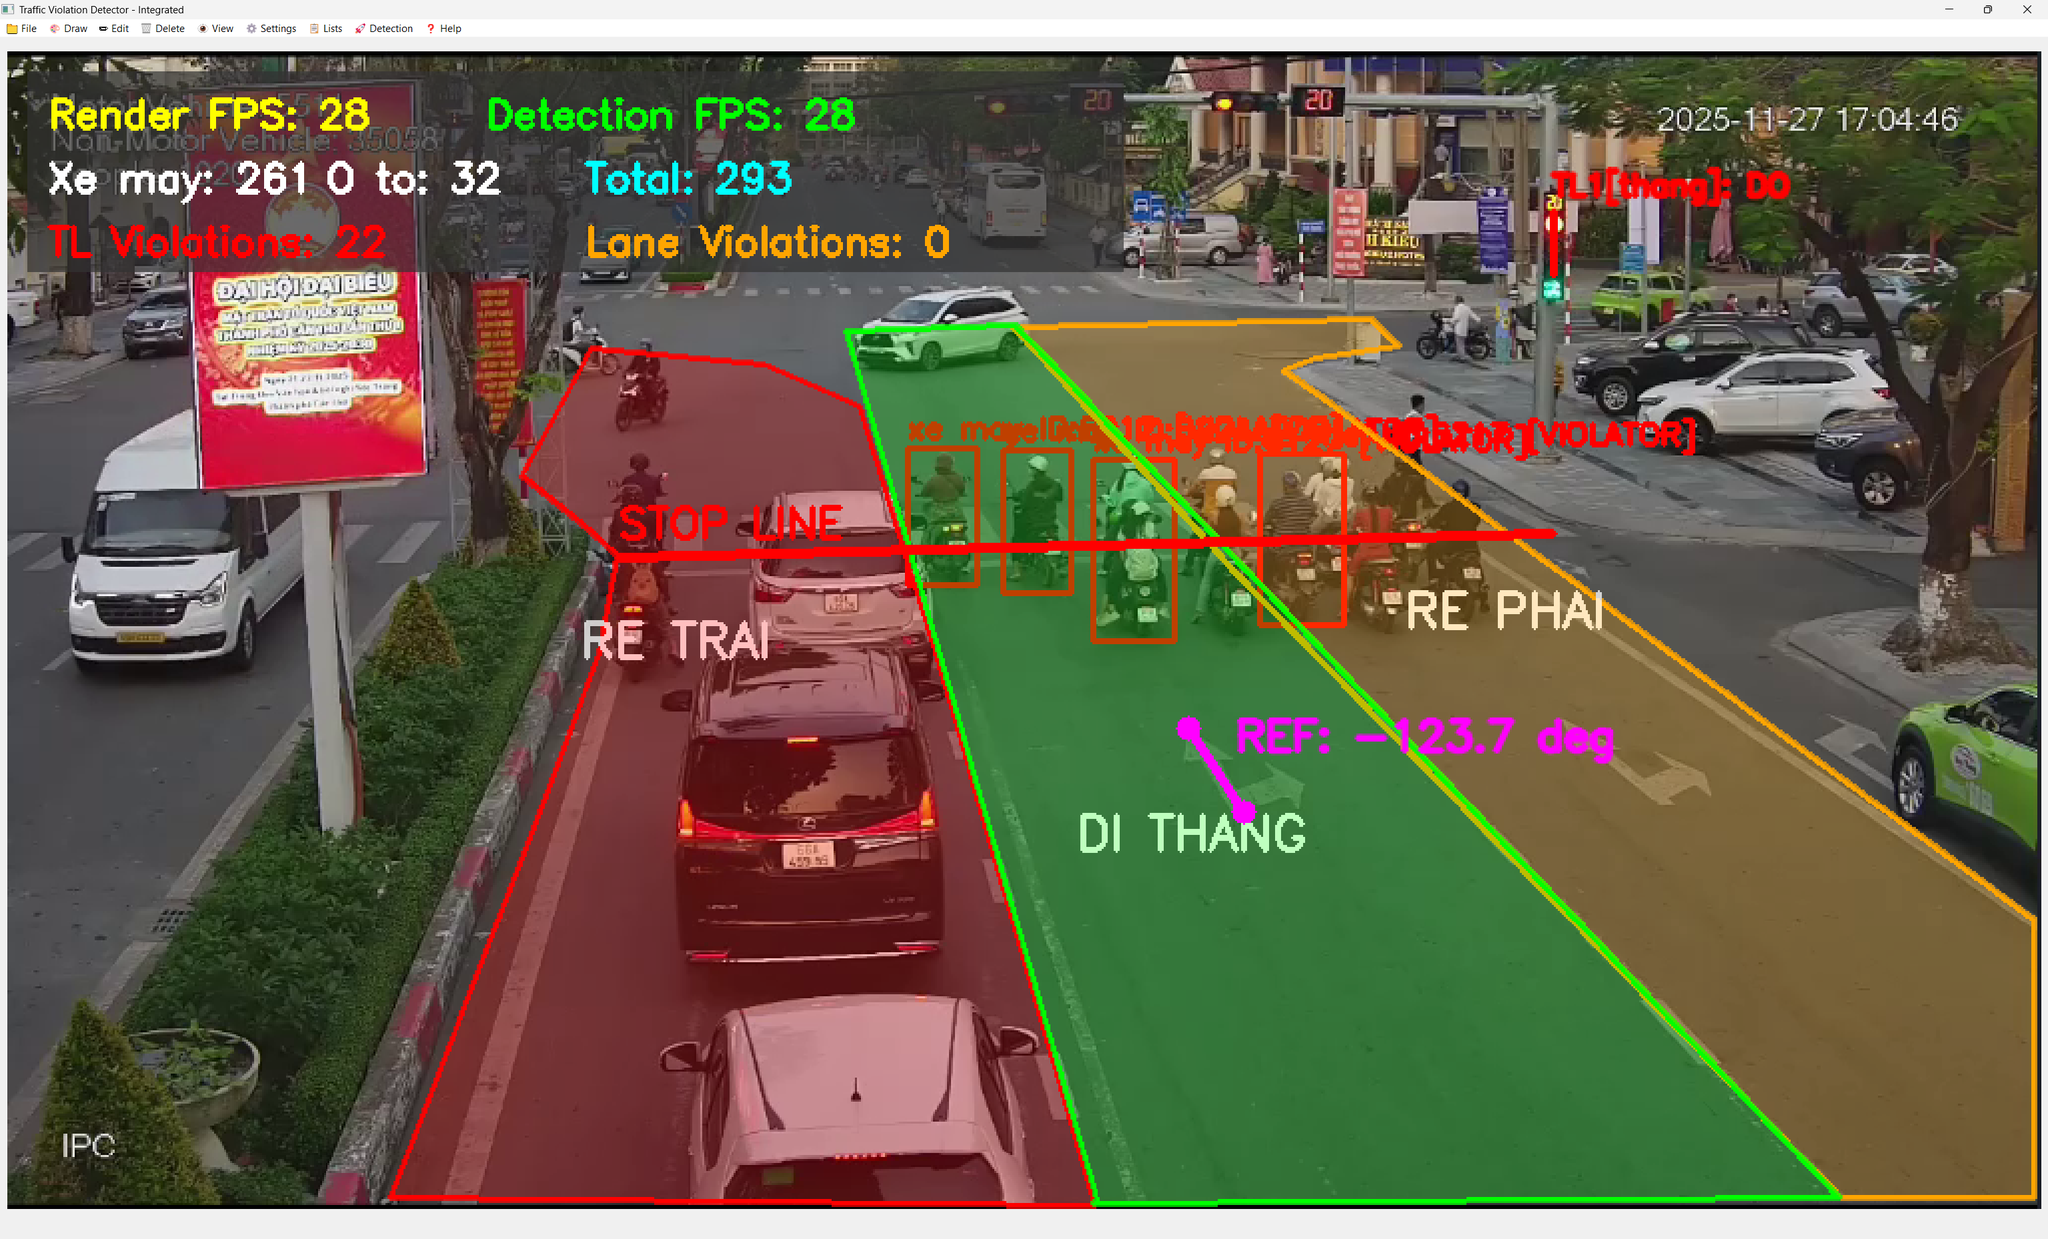
\includegraphics[width=0.7\linewidth]{Figures/inference1.png}
        \caption{Phát hiện xe vượt đèn đỏ (Bbox đỏ = vi phạm)}
    \end{figure}

    \framebreak

    \begin{figure}
        \centering
        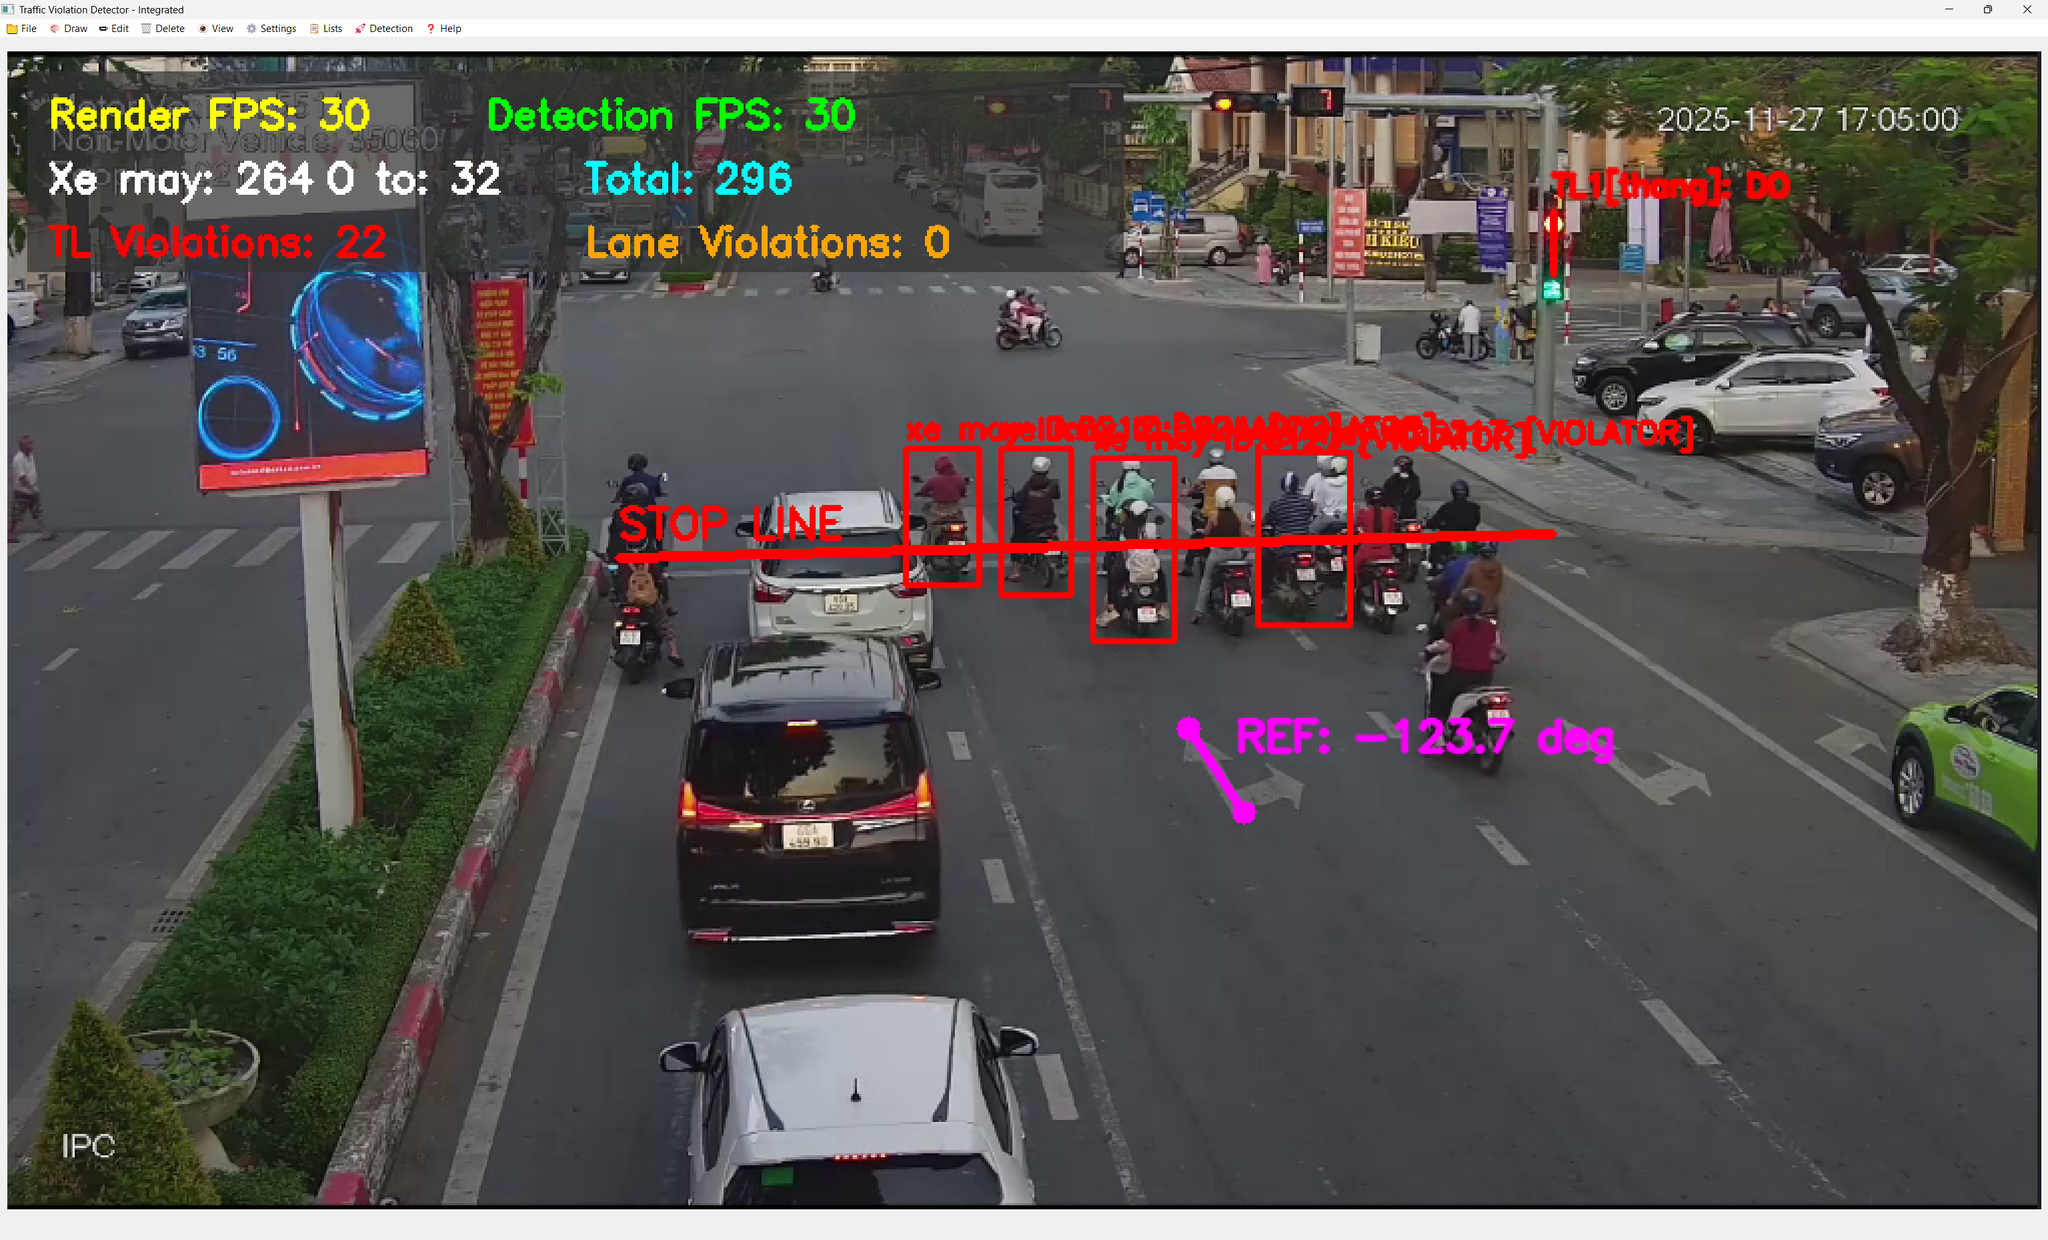
\includegraphics[width=0.7\linewidth]{Figures/inference2.png}
        \caption{Phân loại xe tuân thủ (Bbox xanh) và vi phạm (Bbox đỏ)}
    \end{figure}

    \framebreak

    \begin{figure}
        \centering
        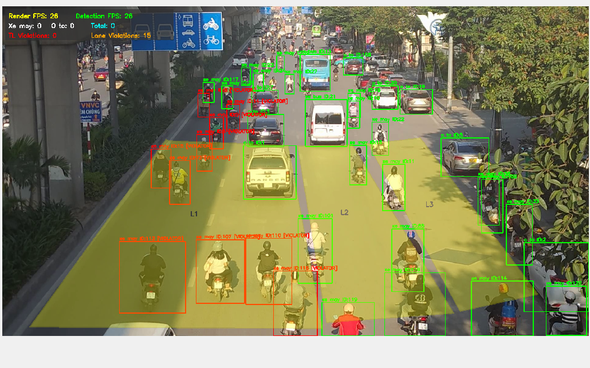
\includegraphics[width=0.7\linewidth]{Figures/inference3.png}
        \caption{Phát hiện xe đi sai làn đường}
    \end{figure}
\end{frame}

%--- ĐÁNH GIÁ HỆ THỐNG ---
\begin{frame}{Đánh giá hệ thống phát hiện vi phạm}
    \begin{block}{Kịch bản 1: Vượt đèn đỏ}
    \begin{itemize}
        \item Logic so sánh tọa độ xe với vạch dừng ảo hoạt động chính xác
        \item Kết hợp với trạng thái đèn (HSV) để đưa ra quyết định
        \item Hỗ trợ 4 loại đèn: Tròn, Rẽ trái, Rẽ phải, Đi thẳng
    \end{itemize}
    \end{block}

    \begin{block}{Kịch bản 2: Đi sai làn}
    \begin{itemize}
        \item Thuật toán Point-in-Polygon xác định xe thuộc làn nào
        \item So sánh loại xe với danh sách cho phép của làn
        \item Hoạt động tốt ngay cả với góc camera thấp
    \end{itemize}
    \end{block}
\end{frame}

%--- THÁCH THỨC VÀ HẠN CHẾ ---
\begin{frame}{Thách thức và Hạn chế}
    \begin{columns}
        \column{0.5\textwidth}
        \textbf{Thách thức đã giải quyết:}
        \begin{itemize}
            \item Mật độ giao thông cao
            \item Điều kiện ánh sáng thay đổi
            \item Đa dạng loại biển số VN
            \item Góc camera nghiêng
        \end{itemize}

        \column{0.5\textwidth}
        \textbf{Hạn chế còn tồn tại:}
        \begin{itemize}
            \item Biển số bẩn/mờ
            \item Biển số nhỏ/xa (Pipeline 2)
            \item Tốc độ giảm khi nhiều xe
            \item Cấu hình ROI thủ công
        \end{itemize}
    \end{columns}
\end{frame}

%--- TỔNG KẾT ---
\begin{frame}{Tổng kết}
    \begin{alertblock}{Kết quả đạt được (theo báo cáo)}
    \begin{itemize}
        \item \textbf{Phát hiện phương tiện:} mAP@50 = \textbf{86.1\%}
        \item \textbf{Phát hiện biển số:} mAP@50 = \textbf{99.5\%} (Pipeline 1)
        \item \textbf{Mô hình tích hợp:} mAP@50 = \textbf{78.5\%} (all classes)
        \item \textbf{Tracking:} ID switches < 5\%
        \item \textbf{Vi phạm:} False positive < 2\%
        \item \textbf{Tốc độ:} 5--20 FPS tùy pipeline
    \end{itemize}
    \end{alertblock}

    \begin{block}{Hướng phát triển}
    \begin{itemize}
        \item Tích hợp auto-retry khi OCR confidence thấp
        \item Hỗ trợ cross-camera tracking
        \item Tự động phát hiện ROI bằng Lane Detection
        \item Triển khai trên edge devices (Jetson)
    \end{itemize}
    \end{block}
\end{frame}

%--- ĐÓNG GÓP ---
\begin{frame}{Đóng góp của đề tài}
    \begin{enumerate}
        \item \textbf{So sánh 2 Pipeline ALPR:}
        \begin{itemize}
            \item Two-Stage: mAP 99.5\%, 5--10 FPS
            \item One-Stage: mAP 78.5\%, 15--20 FPS
        \end{itemize}

        \item \textbf{Huấn luyện 3 mô hình:}
        \begin{itemize}
            \item Model 1: YOLOv8n (5 lớp xe) - mAP 86.1\%
            \item Model 2: YOLOv8n (1 lớp plate) - mAP 99.5\%
            \item Model tích hợp: YOLOv8n (6 lớp) - mAP 78.5\%
        \end{itemize}

        \item \textbf{Hệ thống phát hiện vi phạm:}
        \begin{itemize}
            \item Vượt đèn đỏ (4 loại đèn)
            \item Đi sai làn (Point-in-Polygon)
            \item Direction Fusion (Trajectory + ROI)
        \end{itemize}

        \item \textbf{Ứng dụng:} PyQt5, cấu hình JSON, xuất báo cáo
    \end{enumerate}
\end{frame}

%--- CÂU HỎI ---
\begin{frame}{Câu hỏi thảo luận}
    \centering
    \Huge \textbf{Q\&A}

    \vspace{1em}
    \normalsize
    \textit{Mời thầy cô và các bạn đặt câu hỏi}
\end{frame}
